\section{Conception}
\subsection{Le chassis}
Le chassis est en profile aluminum. Plusieurs solutions se sont %
présentées :\begin{dinglist}{71}%
\item{utiliser du profile pour la construction modulaire}%
\item{utiliser du profile carré}%
\item{utiliser les profiles que propose une célèbre enseigne française %
blanche et verte (fig. \ref{profile} page~\pageref{profile})}
\end{dinglist}%
\par%
\begin{figure}%
   \caption{\label{profile} Profile aluminium 23.5 x 23.5}
   \center{\includegraphics[width=10cm]{img/profile.jpg}}
\end{figure} %
La première solution est chère. Il faut compter 60\euro{} les trois mètres %
(30mm), sans compter la quincaillerie d'assemblage. \par%
La seconde solution, la moins chère, est plus difficile à mettre en %
oeuvre et nécessite de la précision dans les usinages (perçages, sciages, %
...) pour avoir de bons alignements.\par%
La dernière solution est un bon compromis, car c'est une solution de %
construction modulaire à petit prix (15\euro{} les 2,5m x 25mm). Les jonctions %
se font avec des L et des T en PVC. Si ce n'est pas assez rigide, je %
pourrais encore ajouter des équerres métaliques.
\subsection{L'électronique}
\subsubsection{Spécification}
L'électronique de commande doit respecter les spécifications suivantes: %
\begin{dinglist}{71}%
\item{Elle devra piloter 5 axes (1 X-axis, 1 Y-axis, 2 Z-axis, 1 extrudeur)} %
\item{Elle se connectera à un ordinateur via le port USB} %
\item{Elle supportera une carte SD pour l'imprimante soit autonome lors de %
l'impression} %
\item{Elle saura piloter des moteurs pas à pas bipolaires}
\item{Elle intégrera les différents capteurs (fin de course, température de %
l'extrudeur)}
\item{Elle saura piloter le partie chauffante de l'extrudeur} %
\item{Elle ne sera pas propriétaire} %
\end{dinglist} %
\subsubsection{La Smoothieboard}
Toujours, pour des questions de budget, j'ai écarté la solution Smoothie %
(http://smoothieware.org/smoothieboard). Il faut compter 125\euro{} pour une %
carte 5 axes.
\subsubsection{Arduino}
La solution Arduino consiste à utiliser la version Mega et y brancher une carte %
de commande de moteur. Je suis donc parti sur la configuration suivante: %
\begin{dinglist}{71}%
\item{Freeduino 2650 Mega (un clone de l'Arduino, mais en moins cher): 19\euro}%
\item{RAMPS (une carte de commande de moteur; la plus utilisée par les firmwares %
proposés): 14\euro}%
\item{5 modules A4988 (commande de moteur pas à pas) avec radiateur: 5\euro{} chacun}
\end{dinglist}%
%
\subsection{Liste du matériel}
\csvreader[tabular=|l|l|l|r|,
    table head=\hline & Description & Qte & Prix\\\hline,
    late after line=\\\hline]%
{bom.csv}{Description=\Description,Qte=\Qte,Prix=\Prix}%
{\thecsvrow & \Description & \Qte & \Prix}%
%
\subsection{la tête d'impression}
\noindent Fig. \ref{sch_tete} page~\pageref{sch_tete} \par %
\begin{figure}%
   \caption{\label{sch_tete} Dessin de la tête d'impression}%
   \center{\includegraphics[width=5cm]{img/head_sch.jpg}}%
\end{figure}%
La tête d'impression est entièrement fabriquée (fig. \ref{tete_impression} %
page~\pageref{tete_impression}). Elle se compose de quatre éléments:%
\begin{dinglist}{71}%
\item{l'élément de chauffe (qui contiendra la résistance chauffante et la thermistance)}%
\item{le radiateur (qui refroidit la partie haute)}%
\item{le noyau en laiton(pour solidariser le radiateur et l'élément de chauffe)}%
\item{la buse (qui est une partie métalique percée à 0,2mm)}%
\end{dinglist}%
Un noyau en inox (mauvais conducteur thermique) viendra se visser au dessus de la tête.
\begin{figure}%
   \caption{\label{tete_impression} Tête d'impression}%
   \center{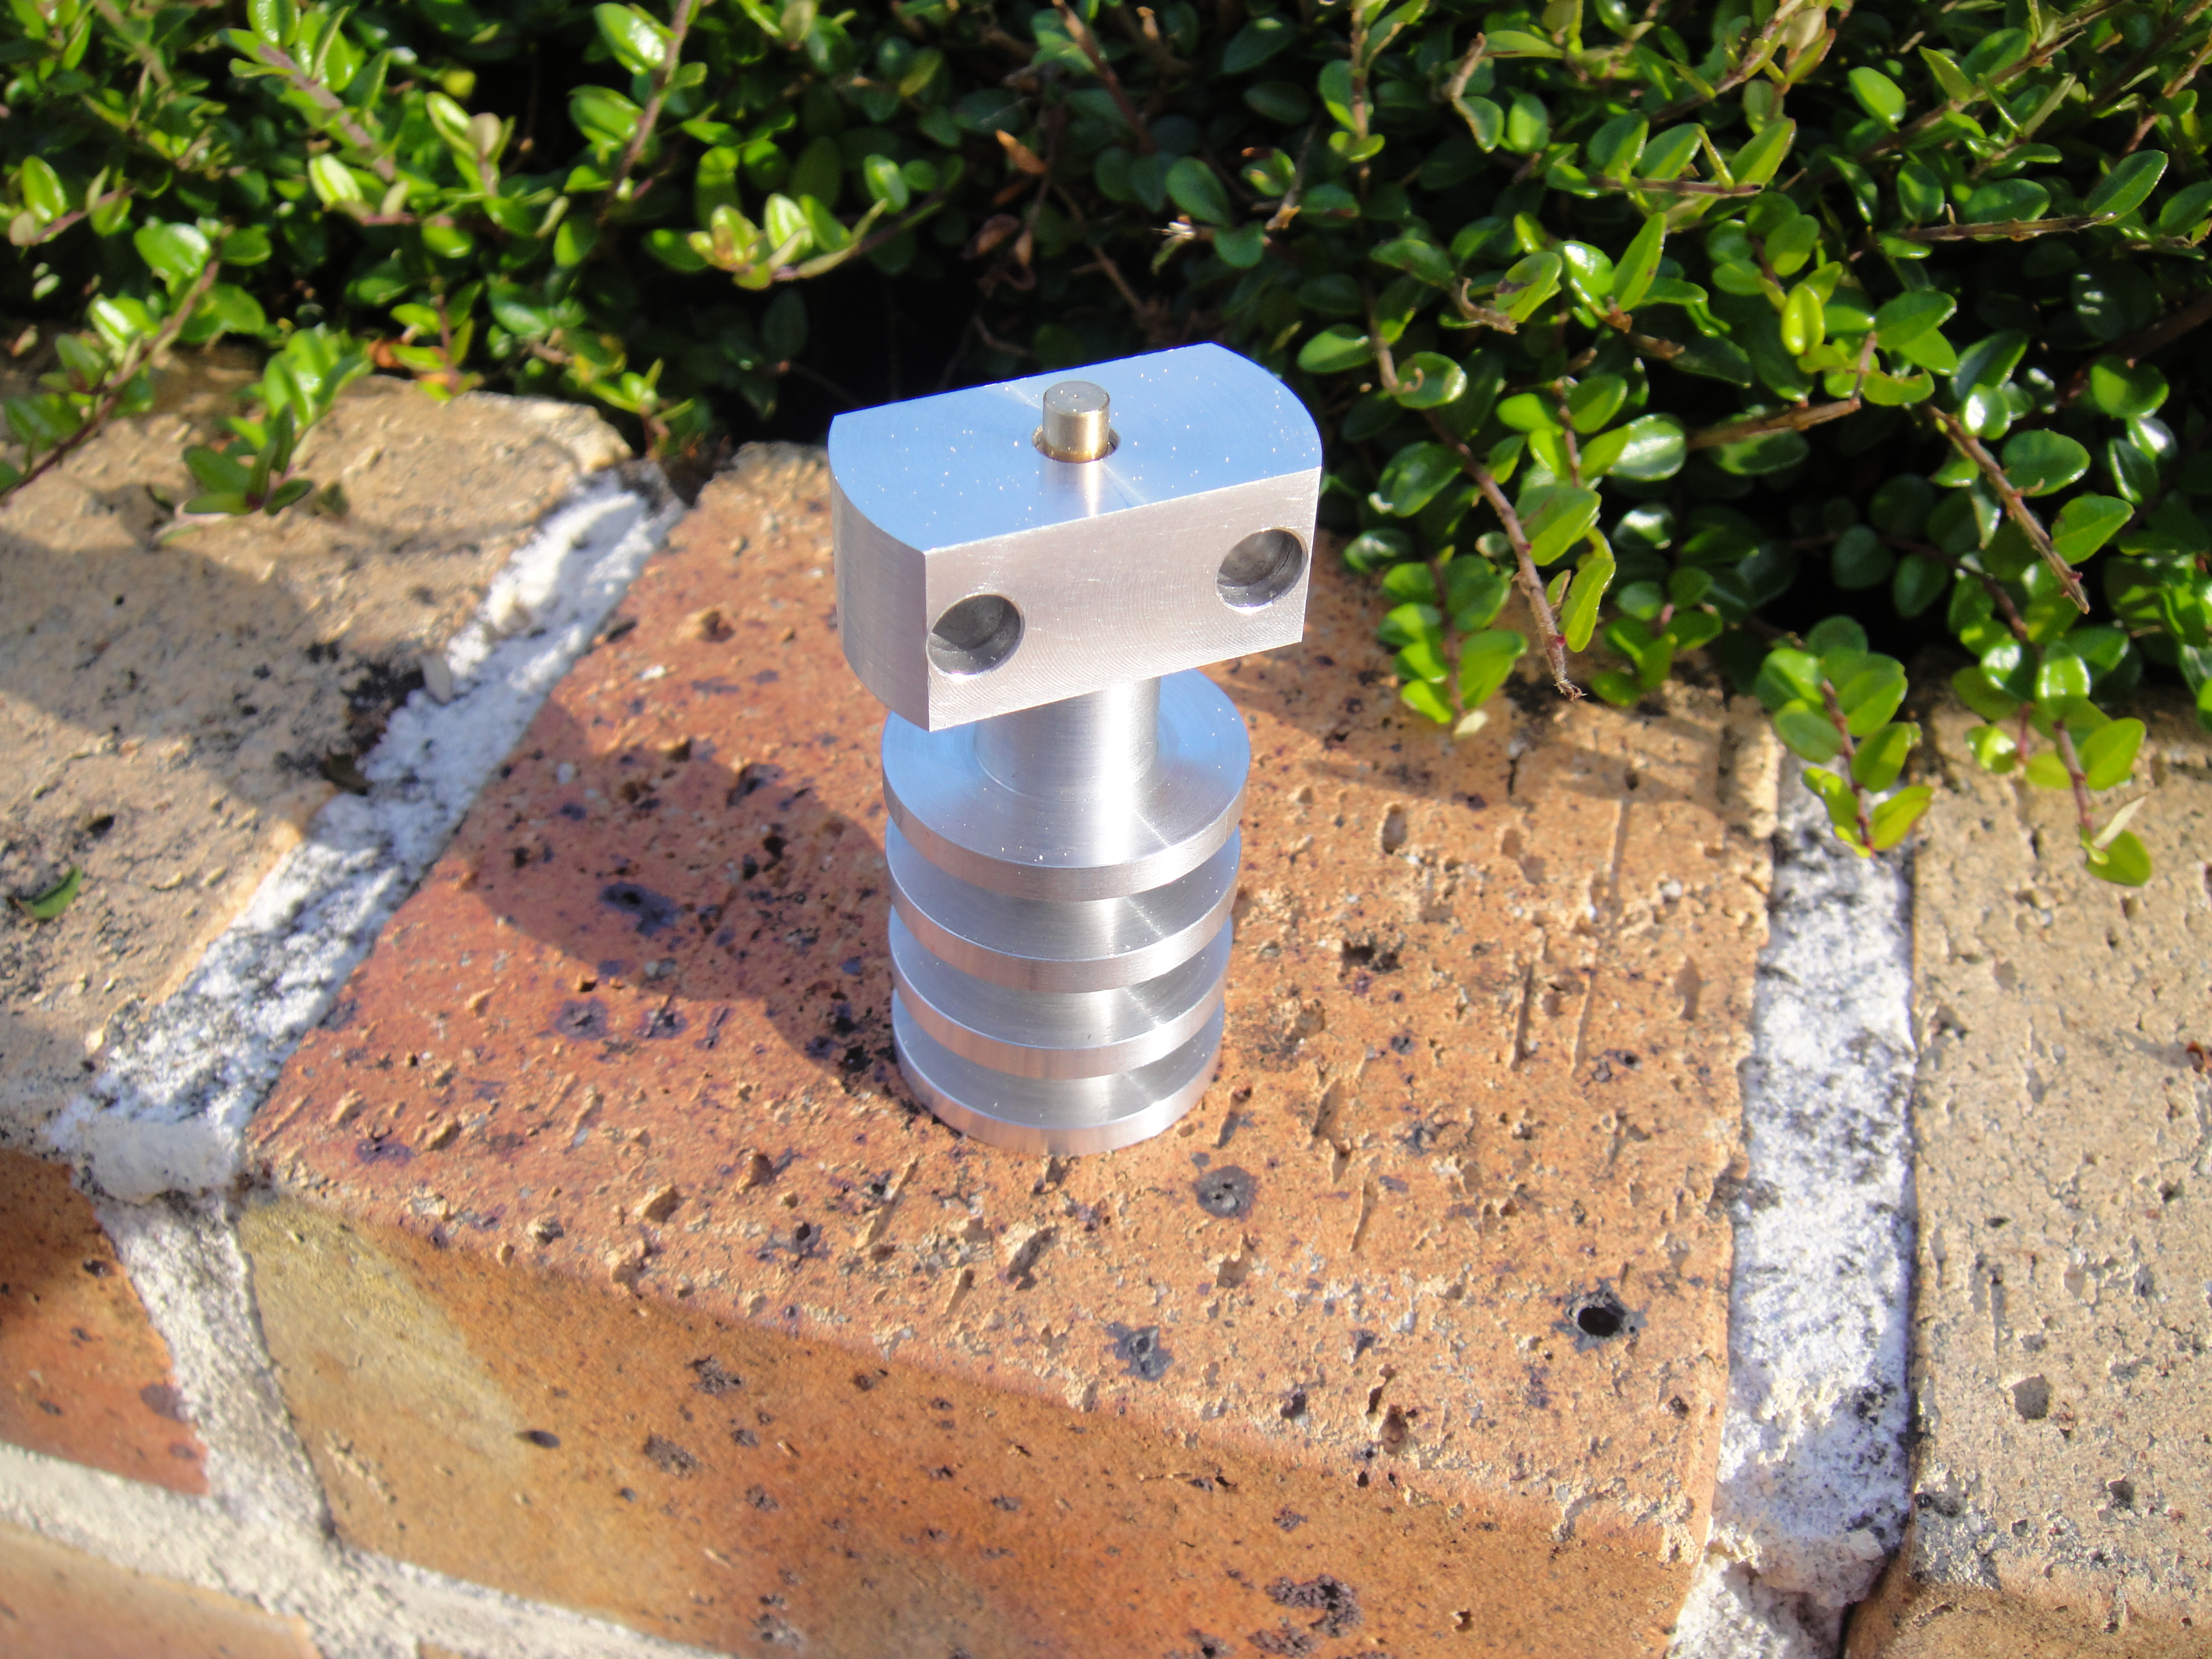
\includegraphics[width=10cm]{img/tete01.jpg}}%
\end{figure}%
\subsubsection{L'élément de chauffe}%
\noindent Fig. \ref{sch_chauffe} page~\pageref{sch_chauffe} \par %
\begin{figure}%
   \caption{\label{sch_chauffe} Dessin de l'élément de chauffage}%
   \center{\includegraphics[width=5cm]{img/heater_sch.jpg}}%
\end{figure}%
La conception est assez simple. Il faut un bloc de métail (dans mon cas de l'aluminium), et %
percer un logement pour la résistance chauffante et un logement pour la thermistance.%
Pour des facilités d'usinage, je suis parti d'un rond d'aluminium que j'ai fraisé %
(fig. \ref{usinage_chauffe} page~\pageref{usinage_chauffe}).%
\begin{figure}%
   \caption{\label{usinage_chauffe} Usinage de l'élément de chauffage}%
   \center{\includegraphics[width=10cm]{img/chauffe01.jpg}}%
\end{figure}%
\subsubsection{Le radiateur}%
\noindent Fig. \ref{sch_radiateur} page~\pageref{sch_radiateur} \par %
\begin{figure}%
   \caption{\label{sch_radiateur} Dessin du radiateur}%
   \center{\includegraphics[width=5cm]{img/cooler_sch.jpg}}%
\end{figure}%
Cette pièce est aussi en aluminium. Avec un tour j'ai usiné des gorges pour faire les ailettes. %
Le perçage central est taraudé à M8 pour y visser le noyau (fig. \ref{usinage_radiateur} %
page~\pageref{usinage_radiateur}).%
\begin{figure}%
   \caption{\label{usinage_radiateur} Usinage du radiateur}%
   \center{\includegraphics[height=8cm]{img/radiateur01.jpg}}%
\end{figure}%
\subsubsection{Le noyau}%
\noindent Fig. \ref{sch_noyau} page~\pageref{sch_noyau} \par %
\begin{figure}%
   \caption{\label{sch_noyau} Dessin du noyau}%
   \center{\includegraphics[width=2cm]{img/core_sch.jpg}}%
\end{figure}%
Le noyau est fabriqué à partir d'une tige fileté M8 en laiton. Cette pièce est percée à 3,2mm %
pour laisser passer le fil de plastique jusqu'à l'élément de chauffe.%
\subsubsection{La buse}%
Le choix de la buse a été assez difficile. La problématique est la suivante : où trouver %
une partie métallique percée à 0,3mm ou moins, pour pas cher ? \par%
Après renseignement, j'ai vite abandonné l'idée de percer moi-même. Les forêts de très petits %
diamètres sont chers et très fragiles (il faut faire des passes de 0,1mm). %
Je me suis rapidement orienté vers les injecteurs de cyclomoteurs ou de gaz. Les injecteurs de %
cyclomoteurs sont percés gros (minimum 0,6mm). Reste les injecteurs gaz. Chez un chauffagiste %
rennais (\url{http://www.jeanpaulguy.fr/contents/fr/p5656_SD_05447200.html}) j'ai trouvé un injecteur de veilleuse de chaudière murale à gaz (fig. \ref{buse} %
page~\pageref{buse}). C'est une petite pièce à moins de 2\euro{}, percée à 0,28mm ou 0,18mm (%
\url{http://www.jeanpaulguy.fr/contents/fr/p2629.html}).%
\begin{figure}%
   \caption{\label{buse} Buse d'extrusion}%
   \center{\includegraphics[width=5cm]{img/buse.jpg}}%
\end{figure}%
\subsection{La platine assemblée}%
\subsubsection{Fixation des glissières à billes}%
Les glissières à billes sont fixées serrées contre la platine. La fixation est usinée dans un premier temps par tournage, en alésant à 15mm un rond d'aluminium. %
La pièce passe ensuite sur le banc d'une fraiseuse pour réaliser les méplats. L'un des méplats sera tangent à l'alésage (en mangeant 0,3mm, pour assurer le serrage %
de la glissière contre la platine. Les perçages de fixation sont taraudés.
\begin{figure}%
   \caption{\label{bushing-bracket} Fixation de glissière à billes}%
   \center{\includegraphics[width=5cm]{img/bushing-bracket.jpg}}%
\end{figure}%
\subsubsection{Fixation et contre-fixation de la courroie}%
Cette pièce est réalisée dans de l'aluminium de 6mm d'épaisseur (ce qui correspond à la largeur de la courroie). Pour créer les dentures, il suffit de percer à d1.5mm %
tous les 2mm (le pas de la courroie est de 2mm). Ensuite, scier le long de la ligne de perçage. On accentuera les dents en passant une lime triangulaire. Les %
perçages de fixation sont fraisurés. Le rayon de courbure de 5mm permet de limiter le frottement de la courroie (le retour risque d'être en contact).
\begin{figure}%
   \caption{\label{belt-blocker} Fixation de la courroie}%
   \center{\includegraphics[width=7cm]{img/belt-blocking.jpg}}%
\end{figure}%
\subsubsection{Montage}%
Commencer par monter la fixation de courroie 2. Monter, sans serrer la contre-fixation 5. Loger les glissière dans leurs fixations et visser ces dernières sur la %
platine (sans trop serrer pour éviter l'hyperstatisme) avec des vis à têtes fraisurées. Il faudra reprendre la fixation des glissières lorsque la platine sera montée %
sur les stubs (barres de glissement).
\begin{figure}%
   \caption{\label{plate-assy} Montage de la platine}%
   \center{\includegraphics[width=16cm]{img/plate-assy.jpg}}%
\end{figure}%
\subsection{Fixation des moteurs}%
Initialement, les moteurs devaient être fixés avec des pièces en platique. Pour des raisons de solidité et de précision, j'ai préféré créer ces pièces en aluminium. %
le centrage des moteurs se fait avec l'alésage de 22mm. Soit cet alésage est réalisé au tour, soit à la lime. Si vous réaliser les alésages au tour, vous n'avez %
pas besoin de les ouvrir à l'extérieur (je l'ai prévu pour laisser passer la lame de scie). Huilez les contacts lors du montage des moteurs afin d'éviter le grippage %
(et abimer les pièces lors d'un prochain démontage). %
La bride de fixation du moteur Y a ses perçages de fixation fraisurés pour assurer un bon contact contre le chassi.
\begin{figure}%
   \caption{\label{y-motor-bracket} Bride de fixation du moteur Y}%
   \center{\includegraphics[width=8cm]{img/y-motor-bracket.jpg}}%
\end{figure}%